\chapter{On Multimedia Analysis and Retrieval}
\epiquote{All our knowledge begins with the senses, proceeds then to the understanding, and ends with reason.}{Immanuel Kant}
\label{chapter:theory_multimedia_analysis_and_retrieval}

This chapter introduces the most important fundamentals on multimedia data, its analysis and the use of derivatives in information retrieval and processing systems. The main sources used in this chapter are the books \emph{Multimedia Retrieval} by H. Blanken et al \cite{Blanken:2007multimedia} and \emph{Similarity Search -- The Metric Space Approach} by P. Zezula et al. \cite{Zezula:2006similarity}, which both provide excellent introductions into the respective fields.

%\epiquote{Quote}{Author}
%%%%%%%%%%%%%%%%%%%%%%%%%%%%%%%%%%%%%%%%%%%%%%%%%%%%%%%%%%%%%%%%%%%%%%%%%%%%%%%%%%%%%

\section{Multimedia Data and Multimedia Collections}
\label{section:multmedia_data}

Multimedia data is ubiquitous and used in different forms in every area of our daily lives, be it private or professional. With the broad adoption of the smartphone in the early 2000s, almost every person on this planet now literally holds the tools required not only to consume but also produce multimedia content in the form of text, images, videos and audio snippets. Fueled by this technological progress, the past few decades have seen a staggering development in both \emph{volume} and \emph{variety} of multimedia data found in the wild, e.g., on the Internet or in personal or professional data collections. 

The term \emph{multimedia} refers to a combination of one or many different \emph{media types}, such as but not limited to, aural or visual information. We distinguish between these types, based on the representation we use when working and interacting with them. Sound, for example, is formed by airpressure waves that are registered by our ears. In contrast, visual information, involves electormagnetic waves captured by our eyes. In both cases, the brain plays an important role in interpreting the underlying processes and forming the human perception of the phenomenon. Similarily, we require different techniques when converting these media types from their analogue to their digital representation. 

Traditionally, we often think of media as information that somehow can be perceived directly by our human senses. However, media data in a wider sense may also include less apparent examples such as motion capture data or data streams stemming from sensors or medical devices. 

At a high level, we can roughly classify all the different media types based on their relationship with time. \emph{Static} media types (e.g., an image) do not exhibit a temporal development, wheras the information in \emph{dynamic} media types (e.g., an audio signal) depends on the time point that is being examined \cite{Blanken:2007multimedia}.

Even though the various media types exhibit very different characteristics in their original representation, we find some commonalities once transfered into the digital domain. These shared properties are crucial for formalising the problem of processing and analysing such data in information processing systems in general and analytics and retrieval systems in particular.

\begin{description}
    \item[Analogue Correspondence] Most digital media types somehow reflect an analogue process taking place in the real-world. Converting such an analogue process to the digital domain requires several steps and intermediate representations, both digital and analogue (see Examples \ref{example:representation_visual_information} and \ref{example:representation_audio_information}).

    \item[Unstructured Data] The raw, digital representation of any media type is typically highly unstructured as opposed to, for example, the highly structured information found in a database. Consequently, we usually do not have natural units of information that can be leveraged directly for analysis. Therefore, information processing system rely on \emph{derivative representations} of the original data, gained through pre-processing and data analysis.
    
    \item[Semantic Gap] The derivative representations of the original data usually describe specific aspects thereof. Conversion between representations is therefore often accompanied by a loss of information, a problem often referred to as the \emph{semantic gap} \cite{Blanken:2007multimedia, Rossetto:2018thesis}.

    \item[Perceptive and Interpretative Gap] Reasoning about the content of any type of media, which is part of the analytical process, requires several steps that involve preception and interpretation of the information by a human consumer. These processes are highly subjective and may lead to different results for different people, adding more indirection in addition to the semantic gap \cite{Rossetto:2018thesis}.
\end{description}

\begin{example}[label=example:representation_visual_information]{Digital Representation of Visual Information}{}
    \begin{wrapfigure}{L}{0.45\textwidth}
        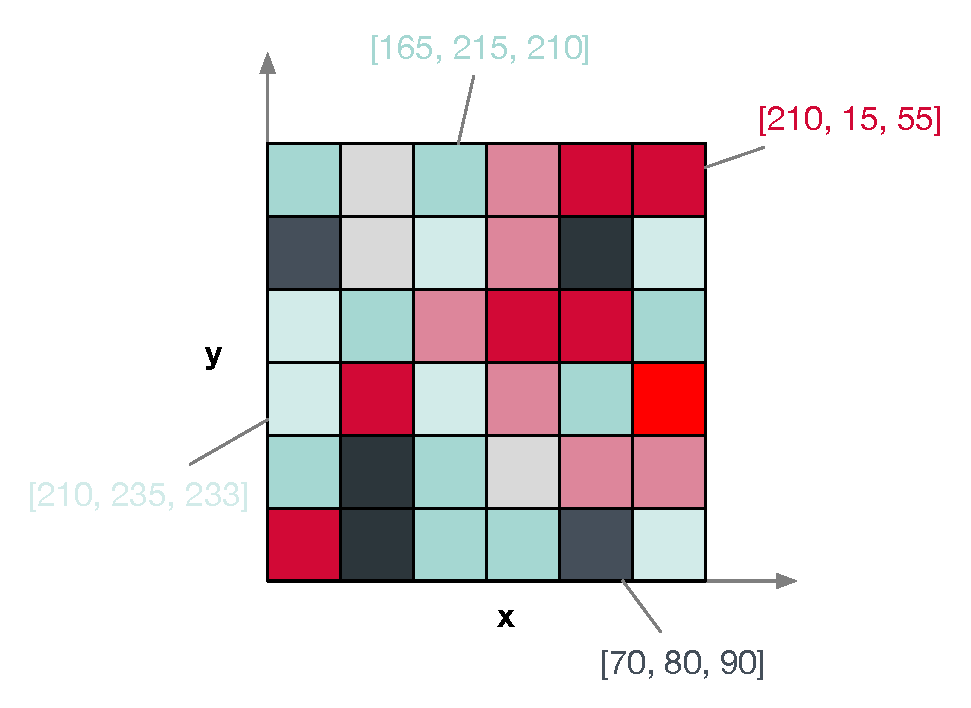
\includegraphics[width=0.45\textwidth]{figures/example-visual-signal.eps}
    \end{wrapfigure}
    The visual information in a flat image is stored as a two dimensional array of \emph{pixels}. The information in every pixel is typically formed by a sensor, in an array of sensors, that captures the electormagnetic signal. Each pixel holds colour values, usually one per colour channel. For example, with the RGB colour model, every pixel holds three values, one for the red, green and blue channel. The number of pixels per dimension determines the \emph{resolution} of the image. Typically, we use a fixed number of bits per colour -- the \emph{colour depth} -- which determines the number colours that can be distinguished.

    If we take, for example, a coloured image of $1000 \times 1000$ pixel, we must encode \num{3e6} individual colour values. Using \SI{8}{\bit} per colour, we end up storing \SI{24e6}{\bit}, which amounts to \SI{3}{\mega\byte} worth of uncompressed image data. Images coming from modern cameras, exhibit resolutions much higher than that.
\end{example}

\begin{example}[label=example:representation_audio_information]{Digital Representation of Aural Information}{}
    \begin{wrapfigure}{R}{0.45\textwidth}
        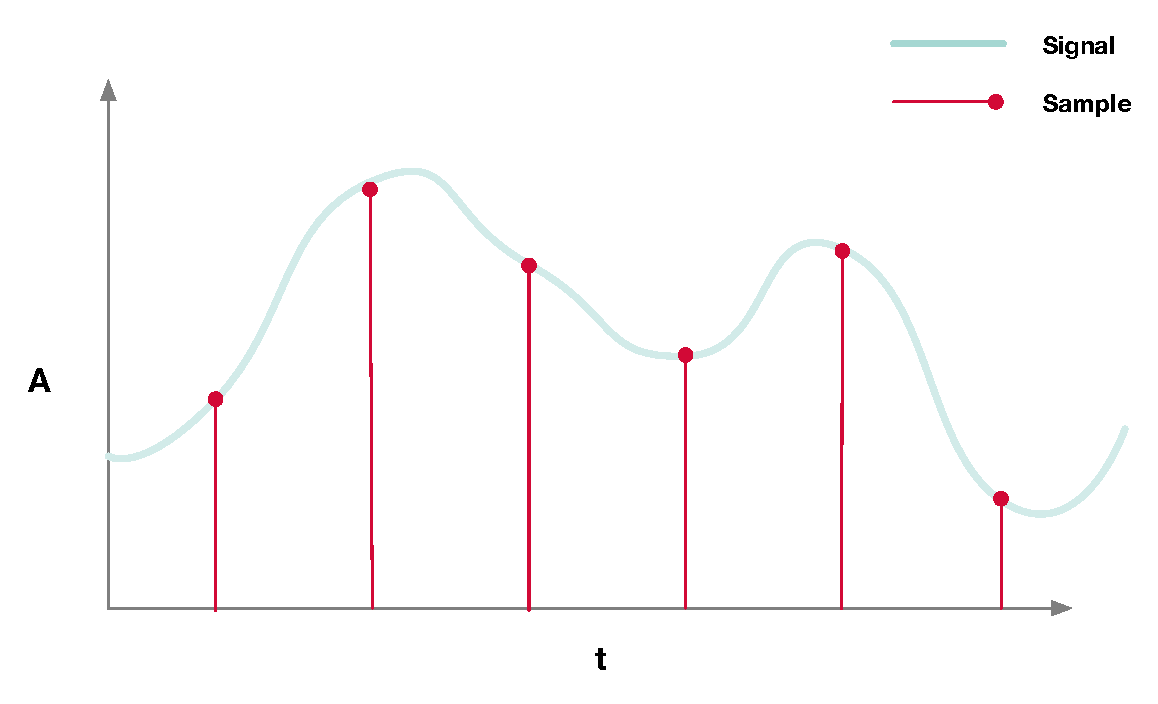
\includegraphics[width=0.45\textwidth]{figures/example-audio-signal.eps}
    \end{wrapfigure}
    The airpressure waves that form sound can be recorded and translated to an electrical signal by microphones. When digitizing this information, the amplitude of such a recorded audio signal is \emph{sampled} at a fixed rate. Each sample point consist of a value that quantizes the amplitude's energy at a given point in time to a number on a given range. An audio stream is then a sequence of these values. The quality of the process is determined by the \emph{sample rate}, i.e., the number of samples per time unit, and the \emph{bit depth}, which determines quantization of the amplitude power.

    If we take a \SI{1}{\second} audio snippet, sampled at \SI{44}{\kilo\hertz}, we end up storing \num{44000} sample points. Using a bit depth of \SI{16}{bit} per sample, this amounts to \SI{704000}{bit} or \SI{88}{\kilo\byte} of uncompressed audio data. In modern audio systems, we typically record multiple audio channels independently, leading to even more data.
\end{example}

\subsection{A Data Model for Media Data}
\label{section:media_data_model}
Despite being agnostic to the concrete, high-level data model in principle, the work presented in this Thesis still relies on a formal understanding of media data that enables organisation and management thereof. Due to its tight integration into the \emph{vitrivr} project \cite{Rossetto:2016vitrivr,Gasser:2019multimodal,Heller:2020multi}, there is a particular model that we would like to introduce. Under this data model -- which is illustrated in \Cref{figure:erm_mediadata_vitrivr} -- a (multi-)media collection consists of multiple \emph{media object}s. The media object describes the data at the level of individual documents -- e.g., a video or image file -- and comprises of basic attributes such its identifier, its media type or its path. The path forms the link to the raw media data in the filesystem, which we assume to be the most suited form of storage for this type of information. 

To account for the temporal development found in dynamic media types, the data model has a notion of a \emph{media segment}, which represents a clearly defined, temporal slice of the object and stands in a one-to-many relationship with it. However, the model does not make any assumption as to how segments are formed. For static media types, such as images, there is a trivial one-to-one relationship between an object and a segment. For more complex media types, such as audio or video, \emph{media segmentation} is a dedicated area of research \cite{Koprinska:2001temporal} and can be approached in many different ways, e.g., at a fixed rate, based on changes in the content \cite{Foote:2000Automatic,Tsai:2016video} or using self-adaptive, deep neural networks~\cite{Souvcek:2019transnet}. Obiviously, different strategies for segmentation yield different degrees of summarization of information over time. Additionally, the proposed distinction also allows for very application specific media types and segmentation strategies, such as \emph{image sequences} -- introduced for \acrshort{lsc} 2020 \cite{Heller:2020Interactive} -- which group related images per day for the purpose of lifelog analysis.

To model the different derivative representations that are used to describe a media object and its segments, the model foresees \emph{features}, which again stand in a one-to-many relationship to the segments. That is, every segment can have an arbitrary number of such features that describe different aspects of the segment's content. In practice, different types of features are obtained and stored in dedicated entities. Additionally, \emph{descriptive metadata} allows for a description of the media both at the document and segment level by means of simple key-value pairs containing descriptions or labels.

\begin{figure}[bt]
    \centering
    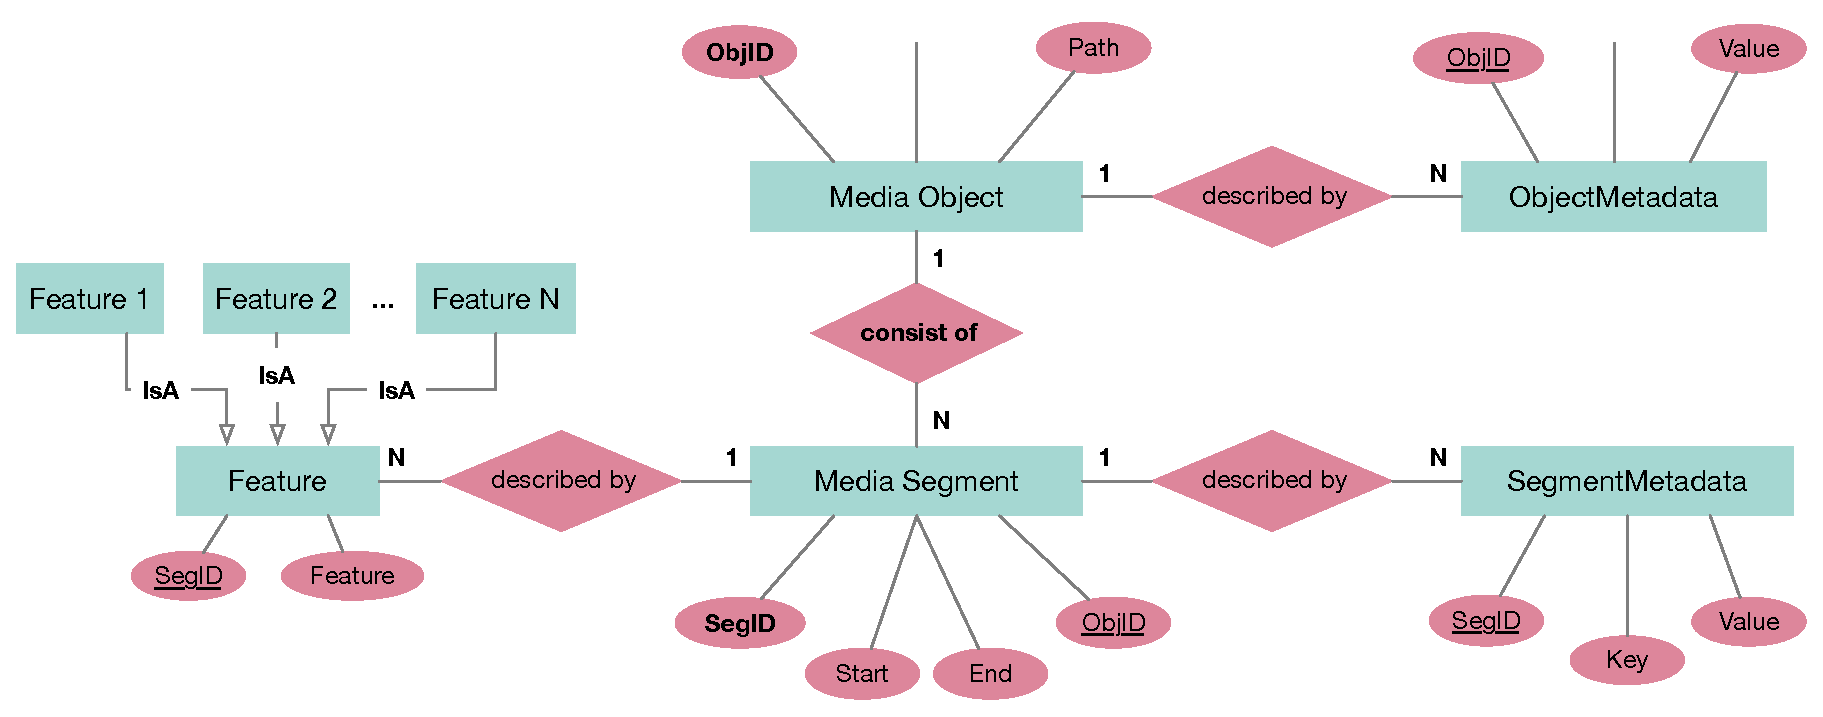
\includegraphics[width=\textwidth]{figures/erm-media-data-vitrivr}
    \caption{An extended \acrshort{erm} of the multimedia data model used in the \emph{vitrivr} project. The model is centered around the notion of media objects and media segments which are described by metadata and features.}
    \label{figure:erm_mediadata_vitrivr}
\end{figure}

While proven to be useful, the proposed model is only one possible approach to model media data and media collections and in  certain aspects, it stands in contrast to \cite{Blanken:2007multimedia}, which considers features to also be a type of metadata. 

For the purpose of this Thesis, we consider a slightly altered version of the aforementioned data model, which is more in line with \cite{Blanken:2007multimedia} and is illustrated in \Cref{figure:erm_mediadata}. It also considers media objects as abbstraction of individual files. However, this model foregoes the indirection introduced by the media segment and treats \emph{features}, \emph{annotations} and \emph{descriptions} as different types of a more general \emph{metadata} type that describes the media object directly. To model the temporal aspect in dynamic media types, the metadata itself exhibits information about the part of the object that is being described, denoted by an optional \emph{start} and an \emph{end} marker. In practice, this could be a frame number or a timestamp.

While the difference between the two models may seem marginal, we argue, that the latter offers several advantages over the former: Firstly, it eliminates a level of indirection introduced by the media segment and thus simplifies handling of static media types, which are simply described by different types of metadata that lack a start and end marker. Secondly, it does not assume segmentation to be statically defined and instead makes this a property of the metadata itself. This is reasonable, because the optimal segmentation strategy may depend on a particular feature, especially when multiple media types must be considered jointly, e.g., aural and visual information in a video. And finally, the model could be easily extended to also support spatial aspects as basis for segmentation, e.g., in images, which would enable it to describe spatio-temporal aspects of any media type. However, such ideas are beyond the scope of this Thesis. 

We will use the proposed model from \Cref{figure:erm_mediadata} throughout this Thesis. Whenever we refer to terms like collection, media object, feature or descriptive metadata, we refer to the concepts introduced in this section.

\begin{figure}[bt]
    \centering
    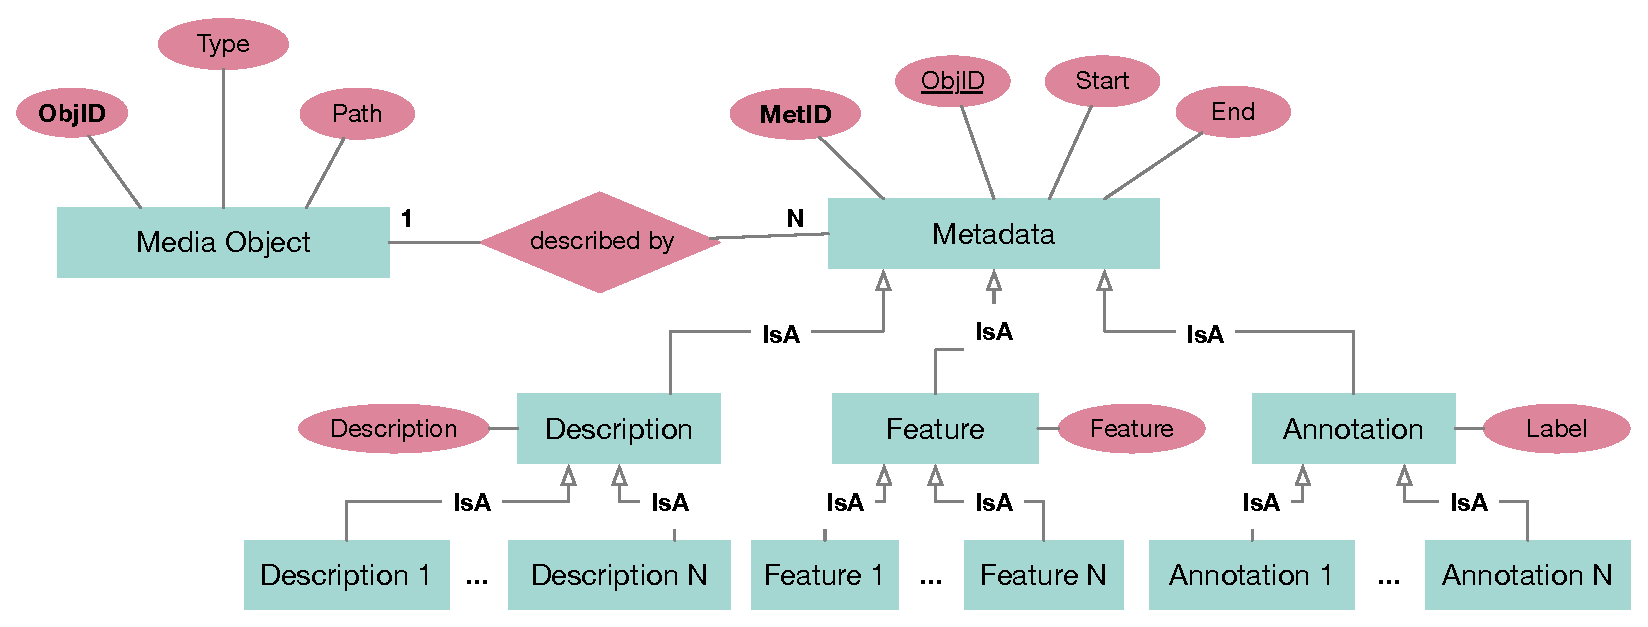
\includegraphics[width=\textwidth]{figures/erm-media-data}
    \caption{An extended \acrshort{erm} of the multimedia data model used for the purpose of this Thesis. It has been derived from \emph{vitrivr}'s data model and foregoes the explicit segment entity.}
    \label{figure:erm_mediadata}
\end{figure}

\subsection{Descriptive Metadata}
Descriptive metadata in the sense of the proposed data model comprises of textual descriptions (e.g, title, summary), technical information (e.g., duration, location, frame rate) and annotations (e.g., category labels). Such information has always played an important role in multimedia retrieval and analysis, because it provides (indirect) access to the media's content and can be leveraged in a structured way, e.g., in database queries or for data organisation.

Over the years, many different metadata standards have emerged. For example, ID3\footnote{See https://id3.org/} tags allow for organisation of large music libraries and classification of songs based on information about artists or albums. Similarily, the Dublin Core Metadata Element Set (DCMES or just Dublin Core)\footnote{See https://www.dublincore.org/} comprises of 15 basic properties that can be used to describe any type of media, e.g., videos or images. And last but not least, EXIF\footnote{See https://www.loc.gov/preservation/digital/formats/fdd/fdd000146.shtml/} can be used to describe images and also includes technical metadata, such as the camera model, the exposure time or the f-number. These well established standards are complemented by umpteenth domain specific, standardised and non-standardised metadata frameworks.

However, while useful and important for the problem of analysis and retrieval, this type of metadata comes with important disadvantages. Firstly, and notwithstanding recent developments in machine learning, e.g., in image captioning \cite{Hossain:2019Comprehensive}, such information is traditionally assigned manually in a laborious and time-consuming annotation process. This process is barely able to keep up with the ever increasing velocity at which new content is created. Secondly, descriptions and labels -- especially if not standardised -- are often subjective due to language, expertise and personal experience and may therefore differ depending on the person assigning them. This is closely related to the problem of the \emph{perceptive- and interpretative gap} \cite{Rossetto:2018thesis}. And finally, it is often challenging to describe the content of media in a textual manner, especially if temporal development is involved.\todo{We use this often. But is there some study on this?}

Regardless of these challenges, however, experience shows that annotations -- be they assigned manually or automatically -- play an important role, especially when it comes to information retrieval. A contributing factor here is that of query formulation, which is very low-effort and familiar for textual input and becomes more challenging for other types of queries \todo{Source}.

\subsection{Features}
Simply put, a \emph{feature} is a mathematical object that describes ``derived characteristics''~\cite{Blanken:2007multimedia} of a media object or a part thereof. Therefore, they are sometimes also referred to as \emph{descriptors}. A bit more formally, given a collection $\mathcal{C} = \lbrace o_1, o_2, \ldots, o_N \rbrace$ of media objects, a \emph{feature} $f \in \mathcal{F}$ describes a temporal interval $[ \texttt{start}, \texttt{end} ]$ with $\texttt{start},\texttt{end} \in \symnatural_0$ of a media object $o \in \mathcal{C}$ under the feature transformation $\phi$, as indicated by \Cref{eq:feature_transformation}. Again, this could be extended to also consider spatial aspects, but the basic concept remains the same.

\begin{equation}
    \label{eq:feature_transformation}
    \phi \colon \mathcal{C} \times \symnatural_0 \times \symnatural_0 \longrightarrow \mathcal{F}
\end{equation}

\cite{Blanken:2007multimedia} distinguishes between low-level and high-level features, which is a qualitative assesment of how far removed the derived characteristic of a particular feature is from a concept that has a semantic meaning to a human user. For example, a histogram of colours would be considered a low-level feature, whereas a feature capturing salient keypoints or even objects in an image would be classified as high-level. In practice, high-level features are often derived from low-level features, and again these conversions are subject to the issue of the semantic gap.

The process of generating features from media objects is called \emph{feature extraction} \cite{Blanken:2007multimedia} and there is an entire corpus of research that deals with the engineering of features that describe the relevant aspects of given media type's content, wherein ``relevant'' is very specific to the particular application or use-case. Various surveys, such as \cite{Ding:2012ASurvey,McKinney:2003Features,Salau:2019Feature}, cover the topic of feature extraction and we simply name and describe a few selected examples to provide an (unrepresentative) overview. 

For images, one can roughly distinguish between low-level colour, texture and shape features \cite{Salau:2019Feature}, as well as higher-level local keypoint-based features. An example of a colour feature could be a simple colour histogram or a statistical moment that captures colour distribution, e.g., the average colour in a defined area of the image. Prominent examples for keypoint detection features include algorithms such as \acrfull{sift}~\cite{Lowe:1999object}, \acrfull{surf}~\cite{Bay:2006surf} or \acrfull{hog}~\cite{Dalal:2005Histograms}. All these features are employed in many different applications ranging from retrieval and similarity search to the detection of higher-level concepts, such as, objects or faces \cite{Deniz:2011Face, Farooq:2016Object}.

Similarily, there is a wide range of features applied in audio analysis and retrieval. \acrfull{mfcc} -- a representation of a short-term power spectrum on the perceptual \emph{mel scale} -- play an important role in speaker recognition, sound and music classification as well as audio segmentation \cite{Kim:2010Comparison} and were shown to outperform audio descriptors outlined in the MPEG-7 standard~\cite{Quackenbush:2001Overview}, which is a collection of standardised ``metadata descriptors'' for images, audio and video. Other types of features include \acrfull{pcp} for music retrieval and classification~\cite{Lee:2006Automatic,Demirel:2019Automatic} or features based on rhythm, timbre or speed.

So far, we have mostly considered features that were engineered through the careful application of signal processing and/or statistical analysis of the raw media data. However, advances in machine learning and deep neural neutwork architectures have enabled the feature extraction process to be automated to some extend, leading to shift from  \emph{engineered} to \emph{learned} features \cite{Hamel:2010Learning,Gordo:2016Deep}. There is also research that deals with the comparison of the two paradigms in multimedia retrieval and analysis \cite{Budnik:2017learned} as well as other domains, such as chemical structure analysis \cite{Gallegos:2021importance}. Preliminary results show, that while learned features often outperform the engineered ones, best results are attained by a combination of the two.

Given the plethora of features and feature extraction techniques for the different types of media, there are two important aspects that ought to be considered with respect to data modeling and data management: First, and despite the vast range of feature extraction techniques, the resulting features often exhibit a comparatively simple mathematical structure. Fir example, we will show in \Cref{section:multimedia_retrieval} that in multimeda retrieval, we very often deal with vectors in a high-dimensional, real-valued vector space \cite{Zezula:2006similarity}. Second, when considering a complex enough use-case, usually no single feature can satisfy all the different types of applications we may encounter because, as we as have pointed out, a specific feature usually focuses on a specific aspect of the content. Consequently, a combination of features often yields the best results \cite{Deselaers:2008Features}.

Both these aspect have important implications for the the requirements on a data management and processing system for multimedia data, especially, if such a system should be able support different use-cases that are not necessarily known in advance. We would also like to point out, that both data models introduced in \Cref{section:media_data_model} can deal with these two aspects.

\section{Multimedia Retrieval}
\label{section:multimedia_retrieval}

\emph{Multimedia retrieval} deals with algorithms, methods and systems that allow for content-based searching and obtaining items of interest from large (multi-)media collections using user-defined queries. Many different research domains for the different types of media have emerged over the years, including but not limited to image retrieval \cite{Dharani:2013Survey}, audio retrieval \cite{Lu:2001Indexing}, video retrieval \cite{Hu:2011Survey}, 3D model retrieval \cite{Yang:2007Content} and various, specialised subdomains \cite{Murthy:2018Content}.

A bit more formal, given an \emph{information need} expressed by a user and transformed into a query $q$, a multimedia retrieval systems aims at finding all media objects $o_j$ contained in the media collection $\mathcal{C}$ that may be relevant to the given information need. This is achieved by obtaining some form of \emph{(dis-)similarity} $s_{q,j}$ between $q$ and $o_j$ and ranking results based on it. This is therefore referred to as \emph{similarity search} and as opposed to Boolean search, the result is not binary in the sense that an object $o_j$ either does or does not match the query. Instead, it matches to a certain degree which is expressed by $s_{q,j}$.

Since usually, direct comparison of media object to a query is not feasible in practice -- for reasons described in \Cref{section:multmedia_data} -- features are used as a proxy instead. This is a manifestation of this concept where derivative representations, i.e., features, are considered in lieu of the actual object itself. The basic flow of information that results from this is illustrated in \Cref{figure:multimedia_retrieval_flow}. 

As described in \Cref{section:media_data_model}, a multimedia retrieval system operates upon features derived from the original media objects. This is done twice: Once when indexing a media object in the collection -- often a step that is thought as taking place offline -- and once when deriving the same feature from the query input provided by the user. Subsequently, the system generates the (dis-)similarity measure for $q$ and $o_j$, which is sometimes converted to a \emph{similarity score} by a correspondence function\footnote{In some cases, the similarity score can also be obtained directly from the features.}. The main advantage of a similarity score is its normalisation to $\left[ 0, 1 \right]$, which makes it more convenient for combining scores when multiple features are considered jointly using, e.g., \emph{score-based late fusion} \cite{Depeursinge:2010Fusion,Rossetto:2018thesis}. 

\begin{figure}[ht]
    \centering
    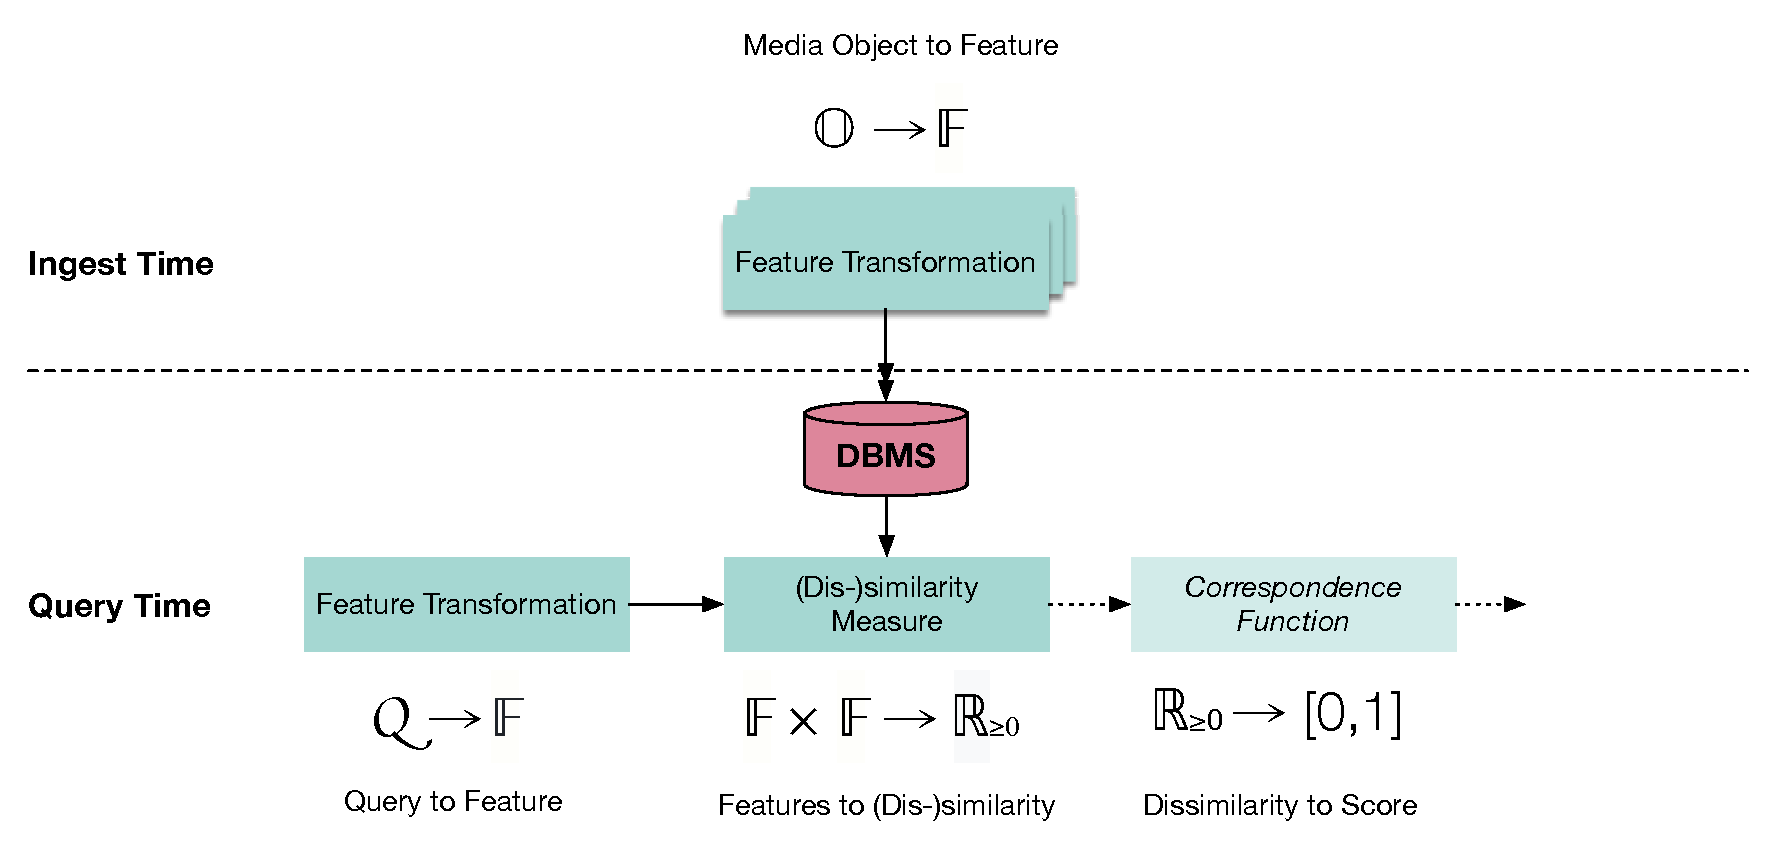
\includegraphics[width=\textwidth]{figures/multimedia-retrieval-pipeline}
    \caption{Flow of information in similarity search at ingest- and query time.}
    \label{figure:multimedia_retrieval_flow}
\end{figure}

\subsection{Similarity Search and the Vector Space Model}

The \emph{vector space model} of similarity search assumes that the domain of the feature vectors $\mathcal{F}$ is a subset of a $d$-dimensional, real-valued vector space, i.e., $\mathcal{F} \subset \symreal^d$. The dimensionality of the vector space is determined by the feature transformation process and may vary between features.

Under this premise, the distance $\delta(f,q)$ between two features $f,q \in \mathcal{F} \subset \symnatural^d$ acts as a proxy for their (dis-)similarity. Typically, the farther two vectors lie apart given a distance function, the more dissimilar they are. Prominent examples of distance functions used in similarity search are listed in \Cref{table:similarity_measures}. 

\begin{table}[hb]
    \begin{tabular}{ | c | c | c | c |}
        \hline
        \textbf{Name} & \textbf{Symbol} & $\mathbf{\delta(f,q)}$ & \textbf{Metric} \\
        \hline
        \hline 
        Manhattan & $L^1$ & $\sum_{i=1}^{d} | f_i - q_i |$ & Yes \\ 
        \hline
        Euclidean & $L^2$ & $\sqrt{\sum_{i=1}^{d} (f_i - q_i)^2}$ & Yes \\  
        \hline
        Minkowski & $L^p$ & $\sqrt[p]{\sum_{i=1}^{d} (f_i - q_i)^p}$ & Yes \\ 
        \hline
        Cosine & - & $1 - \frac{\sum_{i=1}^{d} f_{i}q_{i}}{\sqrt{\sum_{i=1}^{d} f_i^2} \sqrt{\sum_{i=1}^{d} q_i^2}}$ & Yes \\  
        \hline
        Chi-Square & $\chi^2$ & $\sum_{i=1}^{d} \frac{(f_i - q_i)^2}{f_i + q_i}$ & No \\ 
        \hline
        Hamming & - & $1 - \frac{\sum_{i=1}^{d} \min (f_{i},q_{i})}{\sum_{i=1}^{d}  \max (f_{i},q_{i})}$ & No \\
        \hline
    \end{tabular}
    \caption{List of distance functions often used in similarity search for $f, q \in \symreal^d$.}
    \label{table:similarity_measures}
\end{table}

There choice of (dis-)similarity measure mainly depends on the application. All the Minkowski distances, (i.e., $L^1$, $L^2$, $L^p$) are pretty general purpose for any type of real-valued vector and in practice, there it often makes no difference which one is employed \cite{Rossetto:2018thesis}. They all have the advantage, that they induces a \emph{metric} on the underlying vector space, which gives rise to mathematical properties that can be leveraged to optimise query executon. Of all the Minkowski distances, the Euclidean distance ($L^2$) is probably the most common. The Chi-sqaured distance is particularily well suited, if the feature vectors represent histgrams, However, it does no longer induce a metric. The Jaccard- and Hamming-distance when comparing signatures that involve integer numbers or even but patterns, but again with the downside, that they no longer induce a metric.

Regardless of what (dis-)similarity measure is selected, the similarity search problem always looks the same: All features $f_j \in \symreal^d$ are traversed and compared to the query $q \in \symreal^d$ and $\delta(f_j, q)$ is obtained. It then depends on the type of query performed, but generally, we can distinguish between the following three:

\begin{description}
    \item[kNN] The $k$ features $f_j$ for which $\delta(f_j, q)$ is the smallest are retained.
    \item[kFN] The $k$ features $f_j$ for which $\delta(f_j, q)$ is the largest are retained.
    \item[\textepsilon NN] The features $f_j$ for which $\delta(f_j, q) \leq \epsilon$ are retained.
\end{description}

To make the score more practically usable 

Then, depending on the type of similarity search, 

\subsection{Approximate Nearest Neighbor Search}
The nearest neighbor search problem 

\todo[inline]{Describe techniques for approximate nearest neighbor search (ANN). Focus on a more conceptual overview of the types of algorithms rather than just enumerating concrete examples; this can be used as a build-up for discussing properties of different index structures later. }


\subsection{Beyond Similarity Search}
\todo[inline]{Retrieval and analytics techniques that go beyond simple similarity search (e.g. SOM, summarization, clustering)}

\section{Online Multimedia Analysis}
\todo[inline]{Introducing an online analysis pipeline (e.g., Pythia / Delphi).}

\section{Multimedia Analytics}
\todo[inline]{Describe how the combination of analysis }

\subsection{Beyond Similarity Search}

